%!TEX program = xelatex
%!TEX root = ../all.tex

\chapter{Linear classification}

\section*{Introduction to Classification}\label{sec:intro}

The problem of classification represents a fundamental shift from regression tasks we've previously considered. While regression deals with predicting continuous target variables, classification focuses on discrete outcomes. Specifically, in classification problems, the value $t$ we aim to predict comes from a discrete domain where each possible value represents a distinct \alert{class}. The most common scenario involves disjoint classes, meaning each input must be assigned to exactly one class without ambiguity. This requirement leads to a natural partitioning of the input space into \alert{decision regions}, each corresponding to one class.

When we employ \alert{linear classification models}, these decision boundaries take a particularly simple form: they become linear functions of the input $\x$, manifesting as $(d-1)$-dimensional hyperplanes within the $d$-dimensional feature space. This geometric interpretation provides valuable intuition about how classifiers separate different categories. Datasets whose classes correspond to regions that can be separated by such linear decision boundaries are termed \alert{linearly separable}. However, it's important to recognize that real-world data often requires more complex, nonlinear boundaries, which we can achieve through various extensions of these linear models.


%\subsubsection*{Regression vs. Classification: Fundamental Distinctions}
\medskip
Understanding the distinction between regression and classification begins with their output domains. In regression, the target variable $\t$ typically consists of real-valued vectors representing continuous quantities. Classification, by contrast, deals with discrete categories, but offers several representation schemes for these categories.

For binary classification (two classes), we often use a single variable $t\in\{0,1\}$, where $t=0$ denotes class $C_{0}$ and $t=1$ denotes class $C_{1}$. This simple encoding works well for two-class problems. For situations with $K>2$ classes, the most common representation is the \alert{``1-of-$K$'' coding scheme}. Here, $\t$ becomes a vector of $K$ binary elements, where for each class $C_{j}$, all vector elements are 0 except the $j$-th one, which is set to 1. This representation proves particularly useful for extending binary classification methods to multiclass settings.


\subsubsection*{Three Approaches to Classification}

The field of classification offers three principal methodological approaches, each with distinct advantages and theoretical foundations:

\begin{enumerate}
\item The \alert{discriminant function} approach seeks to directly find a function $f:\X\mapsto\{1,\ldots,K\}$ that maps each input $\x$ to its corresponding class label. This approach is appealing in its directness but may lack probabilistic interpretation.

\item The \alert{discriminative approach} operates in two distinct phases. First, during the \emph{inference phase}, we determine the conditional probabilities $p(C_{j}|\x)$ for each class given the input. Then, in the \emph{decision phase}, we use these probability distributions to assign the input to a specific class, typically by selecting the class with the highest posterior probability.

\item The \alert{generative approach} takes a fundamentally different path. Here, we first model the data generation process by determining the class-conditional distributions $p(\x|C_{j})$ along with the class prior probabilities $p(C_{j})$. We then apply Bayes' theorem to derive the posterior probabilities $p(C_{j}|\x)$. Like the discriminative approach, we use these posteriors for classification decisions.
\end{enumerate}

Approaches 1 and 2 are collectively termed \alert{discriminative} because they directly tackle the classification problem by deriving decision boundaries or conditional distributions that discriminate between classes based on the training data. These boundaries are often specified by \alert{discrimination functions} that separate one class from others.

In linear regression, we predict target values using linear functions of the form $h(\x;\w,b)=\w^T\x+b=\ow^T\ox$ (potentially with basis function transformations). For classification, we adapt this framework to predict class probabilities—values constrained to $[0,1]$—through a \alert{generalized linear model} $h(\x;\w,b)=f(\w^T\x+b)$, where $f$ is a nonlinear \alert{activation function} with codomain $[0,1]$.

The decision boundaries in this framework correspond to solutions of $h(\x;\w,b)=c$ for some constant threshold $c$. This yields $\w^T\x+b=f^{-1}(c)$, which represents a linear boundary in the feature space. The inverse function $f^{-1}$ is called the \alert{link function}, connecting the linear predictor to the probability scale.

Approach 3, the \alert{generative} approach, works by defining probabilistic models for items within each class based on training data. These models—probability distributions of features conditioned on class membership—can theoretically be used to generate new synthetic items resembling those in each class. By comparing an unseen item to all class models, we identify the model that best explains the item's features.

%%%%%%%%%%%%%%%%%%%%%%%%%%%%%%%%%%%%%%%%%%%%%%%%%%%%%%%%%%%%%%%%%%%%%%%%%%%%%%%%

\subsection*{Binary Classification with Linear Discriminants}

The equation $\w^T\x + b = 0$ defines a hyperplane in $\mathbb{R}^d$, partioning the space in three regions: the hyperplane itself, and the two half-spaces on either side.

To understand this decomposition, let us consider a point $\x_0$ that lies on the hyperplane, that is such that $\w^T\x_0 + b = 0$. This gives us $b = -\w^T\x_0$, which we can substitute back into the original equation to obtain the equivalent form $\w^T(\x - \x_0) = 0$. Recalling that $\w^T\x$ corresponds to the inner product $\w\cdot\x$ of the two vectors $\w$ and $\x$, this reformulation reveals the hyperplane as the set of all points $\x$ such that the vector $\x - \x_0$ is orthogonal to $\w$. In other words, the weight vector $\w$ is a normal vector with respect to the hyperplane, perpendicular to every vector lying within the hyperplane itself (see Figure \ref{f:hyperplane}).


\begin{figure}[ht]
\begin{center}

\includegraphics[width=8cm]{hyperplane.png}
\end{center}
\caption{Vector view of hyperplane equation.}
\label{f:hyperplane}
\end{figure}


The inner product $\w^T\x$ measures the extent to which $\x$ aligns with the direction of $\w$. When we write $\w^T\x = -b$, we are characterizing the hyperplane as a level set of this linear functional---all points whose projection onto the direction $\w$ yields the constant value $-b$. Geometrically, this means the hyperplane consists of points that share the same signed distance from the origin, measured along the axis defined by $\w$ (see Figure \ref{f:classification_vectors})

To make the notion of distance precise, consider the normalized form of the equation. If $\w \neq \mathbf{0}$, we can divide by $\|\w\|$ to obtain $\frac{\w^T}{\|\w\|}\x + \frac{b}{\|\w\|} = 0$. Here the vector $\frac{\w}{\|\w\|}$ is a unit normal, and the term $\frac{\w^T\x}{\|\w\|}$ represents the length of the orthogonal projection of $\x$ onto the direction of $\w$. The quantity $\frac{|b|}{\|\w\|}$ then gives the perpendicular distance from the origin to the hyperplane, a direct consequence of the fact that the shortest path from the origin to any point on the hyperplane travels along the normal direction (see Figure \ref{f:normalized_distances}).

The sign of $\w^T\x + b$ carries crucial information about which side of the hyperplane a point occupies. For any point $\x$, the value $\w^T\x + b$ is proportional to the signed distance from $\x$ to the hyperplane. When this quantity is positive, $\x$ lies on the side toward which $\w$ points; when negative, it lies on the opposite side. The magnitude $|\w^T\x + b|$ indicates how far $\x$ is from the decision boundary, with larger values representing points more deeply embedded in their respective half-spaces.

The bias term $b$ shifts the hyperplane away from the origin along the direction of $\w$, with the direction of shift determined by the sign of $b$. When $b = 0$, the hyperplane becomes a genuine subspace, passing through the origin and defined purely by the orthogonality condition $\w^T\x = 0$.

In the context of classification, this geometric structure acquires operational significance. The hyperplane acts as a decision boundary, and the inner product $\w^T\x + b$ serves as a discriminant function. For a binary classification problem with labels $t \in \{-1, +1\}$, correct classification occurs when $t(\w^T\x + b) > 0$, meaning the point lies on the correct side of the boundary with some margin. The magnitude of this product measures the confidence of the classification, with larger values indicating greater certainty.


Thus the equation $\w^T\x + b = 0$ encodes a rich geometric structure: a flat subspace defined by orthogonality to $\w$, positioned in space by the bias $b$, and capable of partitioning $\mathbb{R}^n$ into regions based on the sign of the linear functional. The inner product serves as the fundamental mechanism through which this geometric object is defined, analyzed, and utilized for learning.


\begin{figure}[ht]
\begin{center}

\includegraphics[width=8cm]{hyperplane1.png}
\end{center}
\caption{Positive and negative hyperspaces.}
\label{f:classification_vectors}
\end{figure}


\begin{figure}[ht]
\begin{center}

\includegraphics[width=8cm]{hyperplane2.png}
\end{center}
\caption{Normalized distances.}
\label{f:normalized_distances}
\end{figure} 



\subsection*{Multiclass Extension}

When we transition from binary classification to problems involving $K > 2$ classes, the elegant simplicity of a single separating hyperplane becomes insufficient. We require more sophisticated strategies that can partition the feature space into $K$ distinct decision regions, each corresponding to one class. The fundamental challenge lies in how we compose multiple binary decisions to construct a coherent multiclass classifier. We shall examine three distinct approaches to this problem, each with its own geometric characteristics, computational implications, and theoretical limitations. These approaches illustrate important trade-offs between model complexity, interpretability, and the guarantee of obtaining unambiguous classifications.

\subsubsection*{The One-Versus-Rest Strategy}

The most immediate extension of binary classification to the multiclass setting employs what is commonly called the \alert{one-versus-rest} (or \alert{one-versus-all}) strategy. The underlying intuition is straightforward: we train a sequence of binary classifiers, each dedicated to distinguishing one particular class from the aggregation of all remaining classes. Specifically, we define $K-1$ discriminant functions $f_1, f_2, \ldots, f_{K-1}$, where the $i$-th function $f_i$ for $1 \leq i \leq K-1$ is designed to separate points belonging to class $C_i$ from points belonging to any other class.

The decision rule operates as follows. For a given input point $\x$, if $f_i(\x) > 0$, we conclude that $\x \in C_i$. Otherwise, if $f_i(\x) \leq 0$, we infer that $\x \notin C_i$ and belongs to one of the other classes. This sequential testing continues until we encounter a positive response, or we exhaust all $K-1$ classifiers, in which case we assign $\x$ to the final class $C_K$ by default.

While conceptually simple, this approach reveals a fundamental geometric limitation when we examine the structure of the resulting decision regions. The decision boundary for class $C_i$ is determined by the zero level set of $f_i$, but there is no explicit constraint preventing these regions from overlapping or leaving gaps in the feature space. In particular, consider a region where multiple discriminant functions yield positive values simultaneously. Such ambiguities arise naturally because the classifiers are trained independently, without knowledge of each other's decision boundaries. 

\begin{figure}[h]
\centering
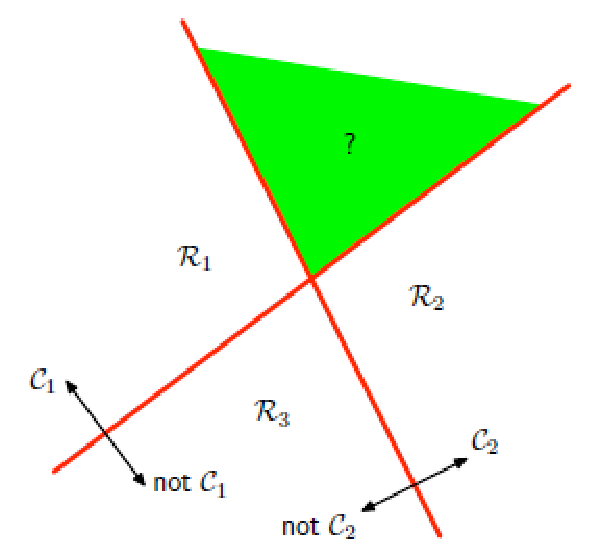
\includegraphics[width=6cm]{figure/fig24.pdf}
\caption{The one-versus-rest approach can lead to ambiguous regions.}
\label{f:1vsall}
\end{figure}

As illustrated in Figure \ref{f:1vsall}, the green shaded region represents points where both $f_1(\x) > 0$ and $f_2(\x) > 0$, meaning such points are claimed by both class $C_1$ and class $C_2$. This overlap indicates a fundamental indeterminacy in the classification: the strategy provides no principled mechanism for resolving which class should take precedence when multiple discriminant functions are positive. Conversely, regions may exist where all $K-1$ discriminant functions are negative yet the point does not naturally belong to class $C_K$, creating additional ambiguity. These geometric pathologies suggest that while the one-versus-rest approach reduces multiclass classification to familiar binary problems, it does so at the cost of potentially incoherent decision boundaries.

\subsubsection*{The One-Versus-One Strategy}

An alternative strategy that addresses some limitations of the one-versus-rest approach is the \alert{one-versus-one} (or \alert{all-pairs}) method. Rather than comparing each class against the collective remainder, we instead train a separate discriminant function for every possible pair of distinct classes. This yields $K(K-1)/2$ discriminant functions $f_{ij}$ where $1 \leq i < j \leq K$, with each function $f_{ij}$ specifically trained to discriminate between class $C_i$ and class $C_j$ in such a way that if $\x$ belongs to class $C_i$, then $f_{ij}(\x) > 0$, whereas if $\x$ belongs to class $C_j$, then $f_{ij}(\x) < 0$. This pairwise comparison provides more focused decision boundaries, as each classifier need only distinguish between two specific classes rather than separating one class from a heterogeneous collection of others.

When classifying a new input $\x$, we employ a majority voting scheme. Each of the $K(K-1)/2$ classifiers casts a vote: for function $f_{ij}$, a positive value votes for class $C_i$ while a negative value votes for class $C_j$. We tally these votes across all pairwise comparisons and assign $\x$ to the class receiving the maximum number of votes. Formally, $\x$ is assigned to class $C_k$ where
\begin{myequation}
k = \arg\max{m} \sum_{j \neq m} \text{sgn}(f_{mj}(\x)),
\end{myequation}
with the understanding that $\text{sgn}(f_{mj}(\x)) = -\text{sgn}(f_{jm}(\x))$ by the antisymmetry of the pairwise discriminant functions.

\begin{figure}[h]
\centering
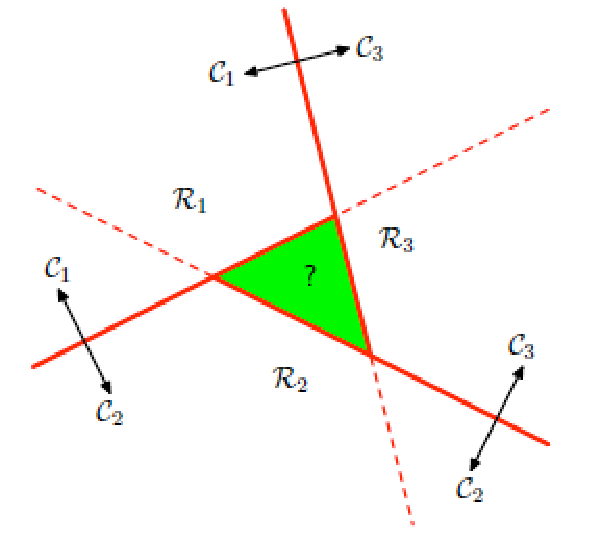
\includegraphics[width=6cm]{figure/fig25.pdf}
\caption{The one-versus-one approach using majority voting can leave regions unassigned.}
\label{f:1vs1}
\end{figure}

Despite its intuitive appeal, this strategy introduces its own geometric complications. Figure \ref{f:1vs1} reveals that certain regions of the feature space may remain unassigned, represented by the green area where the voting results in ties or where no class receives a decisive majority. These unclassified regions represent a different form of ambiguity than the overlaps encountered in the one-versus-rest approach: rather than claiming membership in multiple classes simultaneously, points in these regions are rejected by all classes equally. 

Moreover, the computational cost grows quadratically with the number of classes, as we must train and evaluate $O(K^2)$ classifiers rather than $O(K)$. While each individual classifier operates on a potentially simpler problem involving only two classes, the aggregation mechanism introduces complexity and the possibility of cyclic preferences where classifier $f_{ij}$ prefers $C_i$, $f_{jk}$ prefers $C_j$, and $f_{ki}$ prefers $C_k$, creating Condorcet-style paradoxes in the voting outcomes.

\subsubsection*{The Multiclass Discriminant.}

The third approach, which has become the standard in modern machine learning, abandons the piecewise construction of decision boundaries in favor of a unified framework employing $K$ simultaneous linear discriminant functions. We define for each class $C_i$ a linear function of the form
\begin{myequation}
y_i(\x) = \w_i^T \x + b_i, \quad 1 \leq i \leq K.
\end{myequation}
Each function $y_i$ assigns a real-valued score to every point in the feature space, with higher values indicating stronger evidence for membership in class $C_i$.

The classification rule follows a \alert{winner-take-all} strategy: an input $\x$ is assigned to class $C_k$ if and only if $y_k(\x) > y_j(\x)$ for all $j \neq k$. Equivalently, we select the class index that maximizes the discriminant score:
\begin{myequation}
k = \arg\max{j}{y_j(\x)}
\end{myequation}
This formulation eliminates the ambiguities inherent in the previous approaches by construction: every point in the feature space receives a score from every classifier, and the strict inequality ensures a unique assignment except on a set of measure zero where ties occur.

The geometric structure of the resulting decision boundaries merits careful examination. The boundary separating class $C_i$ from class $C_j$ consists of all points $\x$ where the discriminant scores are equal, that is, $y_i(\x) = y_j(\x)$. Substituting the linear forms yields
\begin{myequation}
\w_i^T \x + b_i = \w_j^T \x + b_j,
\end{myequation}
which rearranges to
\begin{myequation}
(\w_i - \w_j)^T \x + (b_i - b_j) = 0.
\end{myequation}
This equation reveals that the decision boundary between any two classes is itself a $(D-1)$-dimensional hyperplane, where $D$ is the dimensionality of the feature space. The normal vector to this boundary is given by the difference $\w_i - \w_j$, representing the direction in which the relative preference between classes $C_i$ and $C_j$ changes most rapidly. The offset $b_i - b_j$ positions this hyperplane in space according to the relative biases of the two discriminant functions.

The collection of all such pairwise boundaries partitions the feature space into exactly $K$ convex polyhedral regions, each corresponding to one class. This stands in marked contrast to the previous approaches, where regions could overlap or remain unassigned. The argmax formulation guarantees that every point belongs to precisely one decision region (again, except for boundary points of measure zero), providing a complete and unambiguous partition of the input space.

%\section*{Convexity and Connectedness of Decision Regions}

A remarkable property of this approach is that the resulting decision regions are necessarily connected and convex. This geometric regularity has important implications for both the interpretability of the classifier and its robustness to perturbations of the input.

To establish this result formally, consider two arbitrary points $\x_A$ and $\x_B$ that both belong to the same decision region $\mathcal{R}_k$ for class $C_k$. By definition of the decision region, this means that $y_k(\x_A) > y_j(\x_A)$ and $y_k(\x_B) > y_j(\x_B)$ for all $j \neq k$. Now consider any convex combination of these points, $\hat{\x} = \lambda \x_A + (1-\lambda)\x_B$ where $0 \leq \lambda \leq 1$.

The linearity of each discriminant function $y_i$ implies that
\begin{myequation}
y_i(\hat{\x}) = \lambda y_i(\x_A) + (1-\lambda)y_i(\x_B)
\end{myequation}
for all $i$. This linear interpolation property is crucial: the discriminant score at any intermediate point is exactly the weighted average of the scores at the endpoints. Applying this to class $C_k$ and any competing class $C_j$, we have
\begin{myequation}
y_k(\hat{\x}) = \lambda y_k(\x_A) + (1-\lambda)y_k(\x_B) > \lambda y_j(\x_A) + (1-\lambda)y_j(\x_B) = y_j(\hat{\x}),
\end{myequation}
where the inequality follows from the convex combination of the strict inequalities at $\x_A$ and $\x_B$. Thus $y_k(\hat{\x}) > y_j(\hat{\x})$ for all $j \neq k$, establishing that $\hat{\x} \in \mathcal{R}_k$.

This convexity property ensures that the decision region $\mathcal{R}_k$ contains the entire line segment connecting any two of its points. Consequently, the region is not only convex but also connected, meaning there are no disjoint components or ``islands'' belonging to the same class. From a practical perspective, this guarantees that small perturbations of a correctly classified point will not cause abrupt jumps to a different class decision region, contributing to the stability and robustness of the classifier.

\begin{figure}[h]
\centering

\includegraphics[width=6cm]{Figure4-3.pdf}
\caption{The decision regions formed by $K$ linear discriminant functions are convex and simply connected.}
\label{f:convex_decision_regions}
\end{figure}

Figure \ref{f:convex_decision_regions} illustrates this convexity property schematically. The decision boundaries form a Voronoi-like tessellation of the space induced by the linear scoring functions, with each region representing the set of points closer (in a metric induced by the discriminant functions) to one class prototype than to any other. This geometric structure connects the linear discriminant approach to prototype-based classification methods and reveals deep connections to distance metrics in feature space.

\subsubsection*{Comparative Analysis}

Let us compare the three linear multiclass classification strategies introduced above.

The \alert{one-versus-rest} approach is attractive for its simplicity and low computational cost, requiring only $K-1$ binary classifiers. However, this efficiency comes at a geometric price: the resulting decision regions can overlap, leading to incoherent predictions and ambiguous classifications that must be resolved by ad-hoc rules.

The \alert{one-versus-one} approach addresses some of these issues by training a separate classifier for each pair of classes. Each binary decision is more focused and locally meaningful, but this comes with quadratic complexity in the number of classes. Moreover, the combination of pairwise decisions does not guarantee a complete or consistent partition of the feature space, which can result in unclassified or conflicting regions.

By contrast, the \alert{$K$-discriminant argmax formulation} provides a unified and geometrically coherent solution. Its construction yields a complete partition of the feature space into convex, connected regions, with explicit decision boundaries between every pair of classes. The trade-off is that all $K$ weight vectors and biases must be learned jointly, typically by optimizing a multiclass loss function.

This geometric coherence has important consequences for learning. Because each decision region is convex, multiclass classification reduces to a structured form of linear separability: each class is distinguished by the relative ordering of linear scores. This structure supports convex optimization and ensures that, when the data are separable in this multiclass sense, suitable parameters can be found efficiently using algorithms such as multiclass perceptrons or gradient-based methods.


\subsubsection*{Beyond Linearity: Quadratic Discriminants}

A first and conceptually straightforward way to enrich the model consists in explicitly incorporating interactions between pairs of input features. By allowing the classifier to respond not only to individual feature values but also to their joint behavior, one can represent a broader family of decision surfaces. This idea leads to the introduction of \alert{quadratic discriminant functions}, which extend the linear score by adding second-order terms:
\begin{myequation}
h(\x;\w,b)=b+\sum_{i=1}^{d}w_{i}x_i+\sum_{i=1}^{d}\sum_{j=1}^{i}w_{ij}x_ix_j.
\end{myequation}

The structure of this expression deserves some discussion. The first two terms correspond exactly to the affine linear model: a bias term $b$ and a weighted sum of the individual input features $x_i$. The additional double summation introduces all pairwise products $x_i x_j$, including the squared terms $x_i^2$ when $i=j$. Each such interaction is associated with its own parameter $w_{ij}$, allowing the classifier to modulate its response based on how pairs of features jointly vary.

From a parametric perspective, this extension significantly increases the model’s capacity. In addition to the original $d$ weights and the bias term, the quadratic component contributes $\frac{d(d+1)}{2}$ new parameters. While this increase in parameters raises concerns about overfitting and computational cost, it also enables the classifier to represent curved decision boundaries, such as ellipsoids, parabolas, and more general quadratic surfaces.

Geometrically, the inclusion of quadratic terms allows the decision function $h(\x;\w,b)=0$ to define a second-order surface rather than a hyperplane. As a consequence, classes that are not linearly separable in the original feature space may become separable by a quadratic boundary. Importantly, this does not require abandoning the discriminant-function framework: the classifier still assigns labels based on the sign (or relative magnitude) of a single scalar score, preserving much of the interpretability of the linear case.

It is also useful to interpret quadratic discriminant functions as an application of suitable base functions to the original features. The model can be seen as a linear classifier operating in an expanded feature space that includes the original features together with all pairwise products. In this extended space, the decision function remains linear in the parameters, even though it corresponds to a nonlinear boundary in the original input space. This observation anticipates the more general idea of feature transformations and kernel methods, where nonlinear decision boundaries are obtained through linear models applied to suitably chosen representations.


\section*{Least Squares Applied to Classification}

%\subsubsection*{Framework and Interpretation}

The least squares method, typically associated with regression, can be adapted for classification problems. Consider classification with $K$ classes using the 1-of-$K$ coding scheme. This representation uses variables $z_{1},\ldots,z_{K}$, where class $C_{i}$ corresponds to $z_{i}=1$ and $z_{k}=0$ for $k\not=i$.

We derive $K$ discriminant functions $h_i$ as linear regression functions with variables $z_i$ as targets. Each function $h_{i}(\x)=\w_i^T\x+b_i$ is associated with variable $z_i$. We then assign $\x$ to class $C_{k}$ where:
\begin{myequation}
k=\argmax{i}{h_{i}(\x)}
\end{myequation}
Thus, $z_k(\x)=1$ and $z_j(\x)=0$ ($j\not= k$) if $k=\argmax{i}{h_{i}(\x)}$.

A regression function generally estimates the conditional expectation of the target given the input, $\me{t|\x}$. Consequently, $h_i(\x)$ can be interpreted as estimating $\me{z_i|\x}$, the conditional expectation of binary variable $z_{i}$ given $\x$. Assuming $z_i$ follows a Bernoulli distribution, this expectation equals the posterior probability:
\begin{myalign}
h_i(\x)&\simeq\me{z_{i}|\x}\\
&=P(z_{i}=1|\x)\cdot1+P(z_{i}=0|\x)\cdot0\\
&=P(z_{i}=1|\x)\\
&=P(C_{i}|\x)
\end{myalign}
However, we must note that $h_i(\x)$ itself is not constrained to $[0,1]$ and therefore isn't a proper probability measure without further transformation.

\subsubsection*{Learning the Discriminant Functions}

Given a training set $\X,\t$ with $n$ samples, we derive the regression functions via least squares minimization. Each training item is a pair $(\x_{i},\t_{i})$, where $\x_{i}\in\Real^{d}$ and $\t_{i}\in\{0,1\}^{K}$ is the 1-of-$K$ encoded target vector. The predictions $\mathbf{h}(\x_i)=(h_1(\x_i),\ldots,h_K(\x_i))^T$ are computed as:
\begin{myequation}
\y_i=\mathbf{h}(\x_i)=\W\x_i+\mathbf{b}=
 \left(
     \begin{array}{cccc}
          w_{11} & w_{12}  &  \cdots & w_{1d} \\
          w_{21} & w_{22}  &  \cdots & w_{2d} \\
          \vdots &  \vdots & \ddots & \vdots \\
          w_{K1} & w_{K2}  &  \cdots & w_{Kd}  
     \end{array}
     \right)
     \left(
     \begin{array}{c}
          x_{i1} \\
          x_{i2}\\
          \vdots \\
          x_{id} 
     \end{array}
     \right)+
     \left(
     \begin{array}{c}
          b_1 \\
          b_2\\
          \vdots \\
          b_K 
     \end{array}
     \right)
\end{myequation}

To streamline notation, we consolidate all parameters into an augmented matrix:
\begin{myequation}
\overline{\W}=
 \left(
     \begin{array}{ccccc}
          w_{10} & w_{11} &  \cdots & w_{1d} \\
          w_{20} & w_{21}  &  \cdots & w_{2d} \\
         \vdots & \vdots & \ddots & \vdots \\
          w_{K0} & w_{K1} &  \cdots & w_{Kd}  
     \end{array}
     \right)
\end{myequation}
where $w_{i0}=b_i$ for $i=1,\ldots,K$. Similarly, we define the augmented design matrix $\oX\in\Real^{n\times (d+1)}$:
\begin{myequation}
\overline\X=
 \left(
     \begin{array}{cccc}
          1 & x_{11}  &  \cdots & x_{1d} \\
          1 & x_{21}  &  \cdots & x_{2d} \\
          \vdots &  \vdots & \ddots & \vdots \\
          1 & x_{n1}  &  \cdots & x_{nd}  
     \end{array}
     \right)
\end{myequation}

The predictions for the entire training set form a $K\times n$ matrix $\overline\Y$, where column $j$ contains the outputs of all functions applied to $\x_j$:
\begin{myequation}
\overline\Y=
 \left(
     \begin{array}{cccc}
         h_1(\x_1)  &  {h_1(\x_{2})} &{\cdots} & h_1(\x_{n})\\
          h_2(\x_{1})   &  {h_2(\x_{2})} &{\cdots} & h_2(\x_{n})\\
          {\vdots} &  {\vdots} & {\ddots} & {\vdots} \\
          {h_K(\x_{1})}  &  {h_K(\x_{2})} & {\cdots} & {h_K(\x_{n})} 
     \end{array}
     \right)=\overline\W\overline\X^T
\end{myequation}

The target values in 1-of-$K$ format are also represented as a $K\times n$ matrix $\Vbold{T}$, where $\Vbold{T}_{ij}=t_{ji}$, meaning column $j$ is the 1-of-$K$ encoding of target $t_j$:
\begin{myequation}
\Vbold{T}=
 \left(
     \begin{array}{cccc}
          t_{11} &   t_{21} &\cdots &  t_{n1} \\
          t_{12} &   t_{22} &\cdots &  t_{n2} \\
          \vdots &  \vdots & \ddots & \vdots \\
          t_{1K} &   t_{2K} &\cdots &  t_{nK} 
     \end{array}
     \right)
\end{myequation}

The residuals $r_{ij}=h_{j}(\x_{i})-t_{ij}$ form the $K\times n$ residual matrix:
\begin{myequation}
\Vbold{R}=
 \left(
     \begin{array}{cccc}
          r_{11} &   r_{21} &\cdots &  r_{n1} \\
          r_{21} &   r_{22} &\cdots &  r_{n2} \\
          \vdots &  \vdots & \ddots & \vdots \\
          r_{K1} &   r_{2K} &\cdots &  r_{nK} 
     \end{array}
     \right)=\overline\W\overline\X^T-\Vbold{T}
\end{myequation}

Consider the $K\times K$ matrix $\Vbold{R}\Vbold{R}^T$:
\begin{myequation}
\Vbold{R}\Vbold{R}^T=
 \left(
     \begin{array}{cccc}
          \sum_{i=1}^nr_{i1}^2 &   \sum_{i=1}^nr_{i1}r_{i2}&\cdots &  \sum_{i=1}^nr_{i1}r_{iK} \\
          \sum_{i=1}^nr_{i2}r_{i1} &   \sum_{i=1}^nr_{i2}^2&\cdots &  \sum_{i=1}^nr_{i2}r_{iK} \\
          \vdots &  \vdots & \ddots & \vdots \\
         \sum_{i=1}^nr_{iK}r_{i1} &   \sum_{i=1}^nr_{iK}r_{i2}&\cdots &  \sum_{i=1}^nr_{iK}^2
     \end{array}
     \right)
\end{myequation}

The sum of squared residuals across all items and classes corresponds to the trace of $\Vbold{R}^{T}\Vbold{R}$:
\begin{myequation}
\sum_{j=1}^K\sum_{i=1}^{n}(h_{j}(\x_{i})-t_{ij})^{2} = \text{tr}\Big(\Vbold{R}^{T}\Vbold{R}\Big)
\end{myequation}

Thus, we minimize the following objective function:
\begin{myequation}
E({\overline\W})=\frac{1}{2}\text{tr}\Big(\Vbold{R}^{T}\Vbold{R}\Big)
\end{myequation}

Applying standard optimization by solving $\nabla_{\W} E(\overline\W)=\Zero$, we obtain:
\begin{myequation}
\nabla_{\W} E(\overline\W)={\overline \X}^{T}{\overline \X}{\overline\W}-{\overline \X}^{T}\Vbold{T}
\end{myequation}
Setting this gradient to zero yields the closed-form solution:
\begin{myequation}
{\overline\W}=({\overline \X}^{T}{\overline \X})^{-1}{\overline \X}^{T}\Vbold{T}
\end{myequation}

The resulting set of discriminant functions is:
\begin{myequation}
\mathbf{h}(\x)={\overline\W}^{T}{\overline \x}=\Vbold{T}^{T}{\overline\X}({\overline\X}^{T}{\overline\X})^{-1}{\overline\x}
\end{myequation}

This formulation demonstrates how least squares, traditionally a regression technique, can be repurposed for classification by treating class indicators as continuous targets and selecting the class with the highest predicted value. However, this approach has limitations: the predictions are not constrained to valid probability ranges, and the method can be sensitive to outliers and imbalanced class distributions.


\section*{Fisher Linear Discriminant: Maximizing Class Separability}

%\subsection*{The Motivation Behind Linear Discriminant Analysis}

Linear Discriminant Analysis (LDA) represents a fundamental approach to classification that takes a geometric perspective on class separation. Essentially, it is a dimensionality reduction method: however, while dimensionality reduction is usually an unsupervised task, LDA is aimed to be applied into a supervised framework such as classification. The core idea is to transform the feature space through linear projection in such a way that classes become more easily separable. While we've previously discussed linear decision boundaries in the original feature space, LDA operates by finding an optimal subspace—typically of lower dimension—where class discrimination is maximized. This approach is particularly valuable when dealing with high-dimensional data where visualization and interpretation become challenging.

The \emph{Fisher linear discriminant} provides one of the most intuitive and mathematically elegant implementations of this idea. Developed by Ronald Fisher in 1936, this method seeks to find a linear projection that maximizes the separation between classes while minimizing the spread within each class. In its simplest form, Fisher's approach projects all data points from a $D$-dimensional space down to a single dimension through a linear transformation of the form:
\begin{myequation}
y=\w\cdot \x=\w^{T}\x
\end{myequation}
Here, $\w$ represents a $D$-dimensional vector defining the direction of projection. Throughout our discussion, we will consider $\w$ to have unit norm ($\vnorm{\w}_{2}=1$), which simplifies interpretation without loss of generality.

\subsection*{Binary Classification Through One-Dimensional Projection}

For binary classification ($K=2$), once we have projected the data onto the line defined by $\w$, we need only establish a threshold $\tilde y$ to make classification decisions. An item $\x$ is assigned to class $C_{1}$ if its projection $y=\w^{T}\x$ satisfies $y>\tilde y$; otherwise, it is assigned to $C_{2}$. This simple threshold-based classification reduces the $D$-dimensional problem to a one-dimensional decision that can be visualized and analyzed more easily.

\begin{center}

\includegraphics[width=0.5\linewidth]{fisher.pdf}
\end{center}

The effectiveness of this approach depends critically on the choice of projection direction $\w$. Different directions can yield dramatically different levels of class separability, as illustrated in the following examples where the same dataset is projected along four different directions:

\begin{center}
\begin{tabular}{rcl}

\includegraphics[width=0.3\textwidth]{fisher21.pdf}&
 \hspace{2mm}&

\includegraphics[width=0.3\textwidth]{fisher22.pdf}\\

\includegraphics[width=0.3\textwidth]{fisher23.pdf}&
 \hspace{2mm}&

\includegraphics[width=0.3\textwidth]{fisher24.pdf}
\end{tabular}
\end{center}

These visualizations demonstrate that some projection directions preserve class separation better than others. The central challenge of Fisher's method is to find the optimal direction $\w$ that maximizes class separability in the projected space.

\subsection*{Deriving the Optimal Projection Direction for Binary Classification}

\subsubsection*{Initial Intuition: Maximizing Mean Separation}

Let us begin with a straightforward measure of class separation. Given a training set with $n_{1}$ items in class $C_{1}$ and $n_{2}$ items in class $C_{2}$, we first compute the class means:
\begin{myequation}
\mathbf{m}_{1}=\frac{1}{n_{1}}\sum_{\x\in C_{1}}\x\hspace{2cm}\mathbf{m}_{2}=\frac{1}{n_{2}}\sum_{\x\in C_{2}}\x
\end{myequation}

A natural initial criterion for choosing $\w$ would be to maximize the separation between the projected class means. When we project the data onto a line, the projected means become $m_{i}=\w^{T}\mathbf{m}_{i}$, and their separation is:
\begin{myequation}
m_{2}-m_{1}=\w^{T}(\mathbf{m}_{2}-\mathbf{m}_{1})
\end{myequation}

We might initially attempt to maximize this quantity directly. However, we must address two important considerations:

\begin{itemize}
\item The expression $\w^{T}(\mathbf{m}_{2}-\mathbf{m}_{1})$ can be made arbitrarily large simply by scaling $\w$, even though scaling doesn't change the direction of projection. To eliminate this trivial scaling effect, we constrain $\w$ to have unit norm: $\vnorm{\w}_{2}=\w^{T}\w=1$.

\item This leads to a constrained optimization problem:
\begin{myalign}
&\max{\w}\w^{T}(\mathbf{m}_{2}-\mathbf{m}_{1})\\
&\text{subject to }\w^{T}\w=1
\end{myalign}
\end{itemize}

We can solve this problem using Lagrange multipliers, converting it to an unconstrained optimization:
\begin{myequation}
\max{\w,\lambda}\w^{T}(\mathbf{m}_{2}-\mathbf{m}_{1})+\lambda(1-\w^{T}\w)
\end{myequation}

Setting the gradient with respect to $\w$ to zero yields:
\begin{myequation}
\nabla_{\w} (\w^{T}(\mathbf{m}_{2}-\mathbf{m}_{1})+\lambda(1-\w^{T}\w)=\mathbf{m}_{2}-\mathbf{m}_{1}+2\lambda\w=\Zero
\end{myequation}
which implies:
\begin{myequation}
\w=\frac{\mathbf{m}_{2}-\mathbf{m}_{1}}{2\lambda}
\end{myequation}

The constraint $\w^{T}\w=1$ gives us:
\begin{myequation}
\frac{\partial}{\partial\lambda}(\w^{T}(\mathbf{m}_{2}-\mathbf{m}_{1})+\lambda(1-\w^{T}\w))=1-\w^{T}\w=0
\end{myequation}
Solving for $\lambda$, we find:
\begin{myequation}
\lambda=\frac{\vnorm{\mathbf{m}_{2}-\mathbf{m}_{1}}_{2}}{2}
\end{myequation}

Combining these results, we obtain the optimal direction:
\begin{myequation}
\w=\frac{\mathbf{m}_{2}-\mathbf{m}_{1}}{\vnorm{\mathbf{m}_{2}-\mathbf{m}_{1}}_{2}}
\end{myequation}

This solution has an intuitive geometric interpretation: the optimal direction is simply the normalized vector connecting the mean of class $C_1$ to the mean of class $C_2$. While this might seem reasonable at first glance, it has a significant limitation.

\subsubsection*{The Limitations of Mean Separation Alone}

The direction from $\mathbf{m}_{1}$ to $\mathbf{m}_{2}$ maximizes the distance between projected class means, but it doesn't consider how spread out each class is along that direction. Consider the following visualization:

\begin{center}

\includegraphics[width=0.7\textwidth]{fisher.pdf}
\end{center}

Here, while the projected means are well-separated, the classes themselves have high variance along the projection direction, leading to significant overlap in the one-dimensional projection. This overlap would result in many classification errors regardless of where we set the threshold $\tilde y$.

This observation leads us to a crucial refinement: we need to consider not just the separation between class means, but also the \emph{dispersion} or \emph{spread} of each class around its mean. An ideal projection direction should maximize the separation between classes while minimizing the spread within each class.

\subsubsection*{The Fisher Criterion: Balancing Separation and Dispersion}

Fisher’s linear discriminant analysis can be understood as a principled attempt to find a projection of the data onto a one–dimensional axis along which the two classes are as well separated as possible while remaining as compact as possible internally. Rather than focusing only on the distance between class means, Fisher emphasized that a meaningful separation must also take into account how much each class is spread out around its mean. If two classes have very distant means but extremely large variances, their distributions may still overlap substantially after projection, leading to poor classification performance.

To formalize this idea, we consider a projection vector $\w$ that maps any data point $\x\in\Real^d$ onto a scalar $\w^T\x$. In this one-dimensional projected space, we can analyze how each class behaves in terms of both location and dispersion.

\begin{itemize}
\item The \alert{within-class variance} for class $C_{i}$ ($i=1,2$) is defined as:
\begin{myequation}
s_{i}^{2}=\sum_{\x\in C_{i}}(\w^{T}\x-m_{i})^{2}
\end{myequation}
where $m_i=\frac{1}{|C_i|}\sum_{\x\in C_i}\w^T\x$ is the projected mean of class $C_i$.  

This quantity measures how spread out the projected samples of class $C_i$ are around their mean along the direction $\w$. A small value of $s_i^2$ means that most points in class $C_i$ cluster tightly around $m_i$, whereas a large value indicates high variability and significant overlap with the other class after projection.

\item The total within-class variance is then $s_1^2+s_2^2$, which captures the overall dispersion of both classes in the projected space. This term plays a crucial role because excessive spread within either class can blur the boundary between them, even if their means are far apart.
\end{itemize}

\medskip
With these concepts in place, Fisher proposed the following objective function, now known as the \alert{Fisher criterion}:
\begin{myequation}
J(\w)=\frac{(m_{2}-m_{1})^{2}}{s_{1}^{2}+s_{2}^{2}}.
\end{myequation}

The numerator quantifies how far apart the projected class means are, while the denominator quantifies how dispersed the projected classes are. Maximizing $J(\w)$ therefore encourages two complementary effects: large separation between classes and small internal variance within each class. This trade-off is what makes Fisher’s approach particularly effective for linear discrimination.

\subsection*{Matrix Formulation and Optimal Solution}

To derive the optimal projection direction analytically, it is convenient to reformulate the problem using covariance matrices, which capture not only variances but also the geometric structure of the data in the original feature space.

We begin by defining the \alert{within-class covariance matrix} for each class:
\begin{myequation}
\S_{i}=\sum_{\x\in C_{i}}(\x-\mathbf{m}_{i})(\x-\mathbf{m}_{i})^{T},
\end{myequation}
where $\mathbf{m}_i$ is the mean vector of class $C_i$ in the original $d$-dimensional space.  

Each matrix $\S_i$ encodes how points in class $C_i$ vary jointly along different directions. Large values in $\S_i$ indicate directions of high variability, while small values indicate directions where the class is tightly concentrated.

Using this definition, the projected within-class variance can be written compactly as:
\begin{myalign}
s_{i}^{2}
&=\sum_{\x\in C_{i}}(\w^{T}\x-m_{i})^{2}
=\w^{T}\S_{i}\w.
\end{myalign}

This expression makes clear that the variance of the projected data depends not only on $\w$ but also on how the data are distributed in the original space.

\medskip
We then define the \alert{total within-class covariance matrix}:
\begin{myequation}
\S_W=\S_1+\S_2,
\end{myequation}
which summarizes the overall scatter of both classes together.

Next, we introduce the \alert{between-class covariance matrix}:
\begin{myequation}
\S_{B}=(\mathbf{m}_{2}-\mathbf{m}_{1})(\mathbf{m}_{2}-\mathbf{m}_{1})^{T}.
\end{myequation}
This matrix encodes the direction along which the two class means differ. It is rank one, since it is built from a single vector difference.

With these definitions, the squared separation of class means in the projected space becomes:
\begin{myequation}
(m_2-m_1)^2=\w^T\S_B\w,
\end{myequation}
and the Fisher criterion can be rewritten in matrix form as:
\begin{myalign}
J(\w)
=\frac{\w^{T}\S_{B}\w}{\w^{T}\S_{W}\w}.
\end{myalign}

This formulation highlights that Fisher’s problem is a ratio of two quadratic forms: the numerator rewards directions aligned with the difference between class means, while the denominator penalizes directions along which the classes are internally variable.

\medskip
To find the optimal $\w$, we maximize $J(\w)$ by setting its gradient to zero:
\begin{myalign}
\nabla_{\w} \frac{\w^{T}\S_{B}\w}{\w^{T}\S_{W}\w}=\Zero.
\end{myalign}

This leads to the generalized eigenvalue condition:
\begin{myequation}
(\w^{T}\S_B\w)\S_W\w=(\w^{T}\S_W\w)\S_B\w.
\end{myequation}

Noting that $\w^T\S_B\w=c_B$, $\w^T\S_W\w=c_W$, and $(\mathbf{m}_2-\mathbf{m}_1)^T\w=c_m$ are all scalars, we can rewrite this as:
\begin{myequation}
c_B\S_W\w=c_W(\mathbf{m}_2-\mathbf{m}_1)c_m.
\end{myequation}

Solving for $\w$ yields:
\begin{myequation}
\w=\frac{c_Wc_m}{c_B}\S_W^{-1}(\mathbf{m}_2-\mathbf{m}_1).
\end{myequation}

Since only the direction of $\w$ matters (any rescaling produces the same classifier), we discard the scalar factor and obtain the celebrated Fisher solution:
\begin{myequation}
\hat\w=\S_W^{-1}(\mathbf{m}_2-\mathbf{m}_1)
=(\S_1+\S_2)^{-1}(\mathbf{m}_2-\mathbf{m}_1).
\end{myequation}

\medskip
This result has a clear geometric interpretation. The vector $(\mathbf{m}_2-\mathbf{m}_1)$ points from one class mean to the other, indicating the direction of maximum separation in an ideal noise-free scenario. However, the premultiplication by $\S_W^{-1}$ adjusts this direction by accounting for how data are spread in different dimensions. Directions of high variance are down-weighted, while directions of low variance are emphasized. In effect, $\S_W^{-1}$ acts as a whitening transformation that normalizes the data before computing the discriminant direction, ensuring that separation is measured relative to class dispersion rather than absolute distance alone.



\subsection*{Determining the Optimal Threshold}

Once we have found the optimal projection direction $\w$, we still need to determine the threshold $\tilde y$ that will separate the two classes in the one-dimensional projected space. Several approaches exist, but one principled method is to model the class-conditional distributions in the projected space.

\begin{itemize}
\item Assume that the projected values $y=\w^T\x$ for each class follow Gaussian distributions. We can estimate their parameters using maximum likelihood:
\begin{myequation}
m_i=\frac{1}{n_i}\sum_{\x\in C_i}\w^T\x\hspace{1cm}\sigma_i^2=\frac{1}{n_i-1}\sum_{\x\in C_i}(\w^T\x-m_i)^2
\end{myequation}

\item Using Bayes' theorem, we can compute the posterior probability of class $C_i$ given a projected value $y$:
\begin{myequation}
p(C_i|y)\propto p(y|C_i)p(C_i)=p(y|C_i)\frac{n_i}{n_1+n_2}\propto n_ie^{-\frac{(y-m_i)^2}{2\sigma_i^2}}
\end{myequation}

\item The optimal threshold $\tilde y$ can be found as the point where the posterior probabilities of the two classes are equal, or equivalently, where their likelihood ratio equals 1:
\begin{myequation}
\frac{p(C_2|y)}{p(C_1|y)}=\frac{n_2}{n_1}\frac{p(y|C_2)}{p(y|C_1)}=1
\end{myequation}
\end{itemize}

This approach provides a statistically motivated threshold that minimizes classification error under the Gaussian assumption. In practice, if the Gaussian assumption is violated, other methods such as minimizing training error directly or using cross-validation to select the threshold may be more appropriate.

\bigskip

The Fisher linear discriminant, while elegant and intuitive, has certain limitations. It assumes that both classes share the same covariance structure (implied by using a pooled within-class covariance matrix $\S_W$), and it is fundamentally designed for binary classification. Extensions to multiple classes exist but require more sophisticated approaches, such as finding multiple discriminant directions that maximize class separation in a higher-dimensional subspace.

Despite these limitations, Fisher's method remains a cornerstone of pattern recognition and machine learning, providing both theoretical insight and practical utility. Its geometric interpretation makes it particularly valuable for understanding the fundamental challenges of classification and the trade-offs involved in finding optimal decision boundaries.


\section*{Extending LDA to Multiclass Classification}

%\subsection*{The Challenge of Multiple Classes}

Thus far, we have focused primarily on binary classification scenarios where Fisher's Linear Discriminant Analysis (LDA) projects data onto a single dimension. However, real-world classification problems often involve more than two classes, requiring a more sophisticated approach. Extending LDA to multiclass classification presents an interesting challenge: how can we find multiple projection directions that simultaneously maximize separation between all classes?

When $K>2$, we typically assume $D>K$, meaning the number of features exceeds the number of classes. Our goal is to project the original $D$-dimensional data into a $D'$-dimensional subspace, where $1<D'<D$. Rather than a single projection vector $\w$, we now define $D'$ linear transformations:
\begin{myequation}
y_k=\w_k^T\x \hspace{2cm} (k=1,\ldots,D')
\end{myequation}
These transformations collectively project a $D$-dimensional point $\x$ into a $D'$-dimensional point $\y=(y_1,\ldots,y_{D'})^T$. More compactly, if we arrange the projection vectors as columns of a matrix $\W$, the projection becomes:
\begin{myequation}
\y=\W^T\x
\end{myequation}

The fundamental question remains: how do we select these $D'$ projection directions to achieve optimal class separation in this reduced-dimensional space?

\subsection*{Generalizing Covariance Matrices for Multiple Classes}

To extend Fisher's criterion to multiple classes, we must first generalize our definitions of within-class and between-class scatter. Fortunately, the within-class covariance matrix extends naturally to multiple classes. We define:
\begin{myequation}
\S_W=\sum_{i=1}^{K}\S_{i}=\sum_{i=1}^{K}\sum_{\x\in C_{i}}(\x-\mathbf{m}_{i})(\x-\mathbf{m}_{i})^{T}
\end{myequation}
where $\mathbf{m}_{i}$ is the mean vector of class $C_i$:
\begin{myequation}
\mathbf{m}_{i}=\frac{1}{n_{i}}\sum_{\x\in C_{i}}\x
\end{myequation}
This matrix $\S_W$ captures the total spread of data points within their respective classes, regardless of class labels.

Defining the between-class covariance requires more careful consideration. We begin with the total covariance matrix of the entire training set:
\begin{myequation}
\S_{T}=\sum_{\x}(\x-\mathbf{m})(\x-\mathbf{m})^{T}=\sum_{i=1}^{K}\sum_{\x\in C_{i}}(\x-\mathbf{m})(\x-\mathbf{m})^{T}
\end{myequation}
where $\mathbf{m}$ is the overall mean of all training samples:
\begin{myequation}
\mathbf{m}=\frac{1}{n}\sum_{\x}\x=\frac{1}{n}\sum_{i=1}^{K}n_{i}\mathbf{m}_{i}
\end{myequation}

A crucial decomposition emerges when we separate the total covariance into within-class and between-class components:
\begin{myalign}
\S_{T}&=\sum_{i=1}^{K}\sum_{\x\in C_{i}}(\x-\mathbf{m}_{i}+\mathbf{m}_{i}-\mathbf{m})(\x-\mathbf{m}_{i}+\mathbf{m}_{i}-\mathbf{m})^{T}\\
&=\sum_{i=1}^{K}\sum_{\x\in C_{i}}(\x-\mathbf{m}_{i})(\x-\mathbf{m}_{i})^{T} + \sum_{i=1}^{K}\sum_{\x\in C_{i}}(\mathbf{m}_{i}-\mathbf{m})(\mathbf{m}_{i}-\mathbf{m})^{T}\\
&=\S_W+\sum_{i=1}^{K}n_{i}(\mathbf{m}_{i}-\mathbf{m})(\mathbf{m}_{i}-\mathbf{m})^{T}
\end{myalign}

This decomposition reveals that the total covariance $\S_T$ equals the within-class covariance $\S_W$ plus a term quantifying how class means differ from the overall mean. We naturally identify this second term as the between-class covariance matrix:
\begin{myequation}
\S_B=\sum_{i=1}^{K}n_{i}(\mathbf{m}_{i}-\mathbf{m})(\mathbf{m}_{i}-\mathbf{m})^{T}
\end{myequation}

This definition has an intuitive interpretation: $\S_B$ measures the spread of class means around the overall mean, weighted by class sizes. In the binary case, this reduces to our earlier definition $(\mathbf{m}_2-\mathbf{m}_1)(\mathbf{m}_2-\mathbf{m}_1)^T$, scaled appropriately.

%\subsection*{Scatter Matrices in the Projected Space}

When we project the data using $\W$, the scatter matrices in the $D'$-dimensional projected space become:
\begin{myalign}
\mathbf{s}_W&=\sum_{i=1}^{K}\sum_{\x\in C_{i}}(\W^T\x-\overline{\mathbf{m}}_{i})(\W^T\x-\overline{\mathbf{m}}_{i})^{T}\\
\mathbf{s}_B&=\sum_{i=1}^{K}n_i(\overline{\mathbf{m}}_{i}-\overline{\mathbf{m}})(\overline{\mathbf{m}}_{i}-\overline{\mathbf{m}})^T
\end{myalign}
where $\overline{\mathbf{m}}_{i}=\frac{1}{n_i}\sum_{\x\in C_{i}}\W^T\x$ is the projected mean of class $C_i$, and $\overline{\mathbf{m}}=\frac{1}{n}\sum_{\x}\W^T\x$ is the overall projected mean.

A key relationship connects the scatter matrices in the original and projected spaces:
\begin{myequation}
\mathbf{s}_W=\W^{T}\S_W\W \hspace{5mm}\text{and}\hspace{5mm} \mathbf{s}_B=\W^{T}\S_B\W
\end{myequation}
These identities show that the projected scatter matrices are simply linear transformations of the original scatter matrices by the projection matrix $\W$.

\subsection*{Objective Functions for Multiclass LDA}

In multiclass LDA, our goal is to find a projection matrix $\W$ that simultaneously:
\begin{enumerate}
\item Maximizes the dispersion between classes (large $\mathbf{s}_B$)
\item Minimizes the dispersion within classes (small $\mathbf{s}_W$)
\end{enumerate}

Unlike the binary case where we could use a simple ratio, we now need more sophisticated measures to capture these competing objectives across multiple dimensions. Two common approaches emerge:

\begin{enumerate}
\item \textbf{Determinant Ratio Criterion}: This approach considers the ratio of the determinants of the scatter matrices:
\begin{myequation}
J_1(\W)=\frac{|\mathbf{s}_B|}{|\mathbf{s}_W|}=|(\W^{T}\S_W\W)^{-1}\W^{T}\S_B\W|
\end{myequation}
The determinant of a covariance matrix represents the generalized variance (the product of eigenvalues), which in a Gaussian model corresponds to the volume of the distribution. Maximizing this ratio seeks projection directions that maximize the "spread" between classes relative to the "compactness" within classes.

\item \textbf{Trace Ratio Criterion}: An alternative approach uses the trace of the scatter matrix ratio:
\begin{myequation}
J_2(\W)=\text{tr}(\mathbf{s}_W^{-1}\mathbf{s}_B)=\text{tr}{(\W^{T}\S_W\W)^{-1}\W^{T}\S_B\W}
\end{myequation}
The trace of a matrix equals the sum of its eigenvalues, representing the total variance along the principal axes. Maximizing this criterion maximizes the sum of between-class variances relative to within-class variances across all projected dimensions.
\end{enumerate}

Both criteria lead to solutions involving the generalized eigenvalue problem:
\begin{myequation}
\S_B\w_i=\lambda_i\S_W\w_i \hspace{2cm} i=1,\ldots,D'
\end{myequation}
If $\S_W$ is invertible (typically the case when we have more samples than features), this reduces to the standard eigenvalue problem:
\begin{myequation}
(\S_W^{-1}\S_B)\w_i=\lambda_i\w_i
\end{myequation}

The optimal projection matrix $\W^*$ consists of the eigenvectors $\w_1^*,\ldots,\w_{D'}^*$ corresponding to the $D'$ largest eigenvalues $\lambda_1\geq\ldots\geq\lambda_{D'}$.

\subsection*{Dimensionality Considerations in Multiclass LDA}

A crucial theoretical result in multiclass LDA is that the between-class scatter matrix $\S_B$ has rank at most $\min(K-1, D)$. This follows because $\S_B$ is formed from $K$ class means, and the overall mean is a linear combination of these means. Consequently, there are at most $K-1$ linearly independent directions along which class means can vary.

This leads to an important practical constraint: the maximum number of meaningful discriminant directions we can extract is $K-1$. In practice, we typically set $D'=K-1$, as projecting to a higher-dimensional space would not provide additional discriminatory power (the additional eigenvalues would be zero).

Thus, multiclass LDA effectively reduces the dimensionality from $D$ to at most $K-1$, which can be a dramatic reduction when dealing with high-dimensional data with few classes.

\subsection*{Practical Implementation and Interpretation}

The implementation of multiclass LDA involves several steps:
\begin{enumerate}
\item Compute the within-class scatter matrix $\S_W$ and between-class scatter matrix $\S_B$ from the training data.
\item Solve the generalized eigenvalue problem $\S_B\w=\lambda\S_W\w$.
\item Sort eigenvalues in descending order and select the eigenvectors corresponding to the $K-1$ largest eigenvalues.
\item Form the projection matrix $\W$ from these eigenvectors.
\item Project all data points: $\y=\W^T\x$.
\end{enumerate}

The resulting projection directions have interesting geometric interpretations:
\begin{itemize}
\item The first discriminant direction ($\w_1$) provides the maximum separation between all classes.
\item Subsequent directions ($\w_2, \w_3, \ldots$) provide additional separation orthogonal to previous directions.
\item These directions maximize class separability in the projected space while decorrelating the projected features.
\end{itemize}

\subsection*{Limitations and Considerations}

While multiclass LDA is a powerful technique, several limitations warrant consideration, such as

\begin{itemize}
\item When the number of samples $n$ is less than the number of features $D$, $\S_W$ becomes singular and non-invertible. Regularization techniques or dimensionality reduction methods (like PCA) may be required as preprocessing steps.

\item LDA assumes each class follows a Gaussian distribution with equal covariance matrices. When these assumptions are violated, quadratic discriminant analysis (QDA) or other nonlinear methods may be more appropriate.

\item LDA finds linear projection directions. For complex, nonlinear class boundaries, kernel extensions (Kernel LDA) or other nonlinear methods may be necessary.

\item The between-class scatter matrix $\S_B$ weights each class by its size $n_i$. In imbalanced datasets, this may cause the projection to be dominated by larger classes.
\end{itemize}

Multiclass LDA is also particularly valuable for visualization. By projecting high-dimensional data onto the first two or three discriminant directions, we can create 2D or 3D scatter plots that reveal the inherent class structure of the data. 

\begin{figure}[ht]
\begin{center}

\includegraphics[width=0.6\linewidth]{multiclass_lda_example.png}
\end{center}
\caption{Separation of three classes in 2D via LDA.}
\label{f:lda3c}
\end{figure}


Figure \ref{f:lda3c} illustrates how multiclass LDA can successfully separate three classes in a two-dimensional projection, even when the original data resides in a much higher-dimensional space.

\section*{Perceptron}

The perceptron was introduced in the 1960s and is widely regarded as one of the foundational models of the neural network paradigm. Historically, it represented one of the first attempts to formalize learning in artificial systems inspired by biological neurons. Despite its conceptual simplicity, the perceptron played a crucial role in shaping subsequent developments in machine learning and artificial intelligence.

At its core, the perceptron is a very simple mathematical abstraction of a single neuron. It takes a vector of inputs and produces a binary output by computing a weighted sum of those inputs, possibly including a bias term, and then applying a nonlinear decision function. Because of this structure, it is often described as a linear classifier with a hard threshold.

From a probabilistic perspective, the perceptron is difficult to interpret, since it does not explicitly model uncertainty or class probabilities. Instead, it provides a deterministic decision based solely on the sign of a linear function. Moreover, a well-known limitation of the perceptron is that it can only correctly classify data that are linearly separable, meaning that there must exist a hyperplane that perfectly divides the two classes. If such a hyperplane does not exist, the standard perceptron learning algorithm will fail to converge.

Formally, the perceptron corresponds to a binary classification model in which an input vector $\x$ is assigned to one of two classes based on the sign of a linear combination of its components. Specifically, the model is defined as
\begin{myequation}
h(\x)=f(\w^T\x+b)=f(\ow^T\ox)
\end{myequation}
where $\w$ is the weight vector, $b$ is a bias term, and $\ow$ and $\ox$ denote the augmented vectors including the bias. The function $f(\cdot)$ is the sign function, defined as
\begin{myequation}
f(i)=
\begin{cases}
-1 & \text{if } i< 0\\
1 & \text{if } i\geq 0
\end{cases}
\end{myequation}
This means that the perceptron divides the input space into two half-spaces separated by a hyperplane. In this sense, the perceptron can be seen as a particular instance of a generalized linear model, albeit with a very specific and non-smooth activation function.

Because of this definition, the output of the model $h(\x)$ can only take the values $\pm 1$. We interpret $h(\x)=1$ as assigning $\x$ to class $C_{1}$ and $h(\x)=-1$ as assigning $\x$ to class $C_{2}$. In a supervised learning setting, each training example $\x_i$ is therefore associated with a target label $t_i\in\{-1,1\}$ indicating its true class membership.

\medskip
A natural first idea for a cost function would be to count the number of misclassified elements in the training set. However, this leads to a piecewise constant objective function that is flat almost everywhere. As a consequence, gradient-based optimization methods cannot be applied, since the gradient is zero for almost all parameter values.

To overcome this issue, one introduces a different cost function that is continuous and piecewise linear in the parameters. The intuition is that we do not only want to penalize misclassified points, but also take into account how badly they are misclassified.

Ideally, we would like to find a weight vector $\w$ such that for every training example $\x_i$,
\begin{myequation}
\ow^{T}\ox_i>0 \quad \text{if } \x_i\in C_{1}, \qquad 
\ow^{T}\ox_i<0 \quad \text{if } \x_i\in C_{2}.
\end{myequation}
Equivalently, using the target labels, this condition can be written compactly as
\begin{myequation}
\ow^{T}\ox_i t_i>0
\end{myequation}
for all $i$. This expresses the requirement that the model not only classifies correctly, but does so with a positive margin.

\medskip
Each training example contributes to the cost function depending on whether it is correctly classified or not. If $\x_i$ is correctly classified, its contribution is zero. If instead it is misclassified, its contribution is given by the positive quantity $-\ow^{T}\ox_i t_i$. Let $\cal M$ denote the set of all misclassified elements. The overall cost function can then be written as
\begin{myequation}
E_{p}(\ow)=-\sum_{\x_{i}\in{\cal M}}\ow^T\ox_it_i.
\end{myequation}
This expression makes clear that only misclassified points affect the cost, and that their influence depends linearly on the current parameters $\ow$.

To minimize this cost function, one can apply gradient descent. Starting from an initial guess $\ow^{(0)}$, the parameters are updated iteratively according to
\begin{myequation}
\ow^{(k+1)}=\ow^{(k)}-\eta\nabla_{\ow} E_{p}(\ow)\Big|_{\ow^{(k)}},
\end{myequation}
where $\eta>0$ is a learning rate controlling the step size. The gradient of the cost function with respect to $\ow$ is
\begin{myequation}
\nabla_{\ow} E_{p}(\ow)=-\sum_{\x_{i}\in{\cal M}}\ox_i t_i.
\end{myequation}
Substituting this into the update rule yields
\begin{myequation}
\ow^{(k+1)}=\ow^{(k)}+\eta\sum_{\x_{i}\in{\cal M}_{k}}\ox_i t_i,
\end{myequation}
where ${\cal M}_{k}$ denotes the set of points misclassified by the model at iteration $k$.

In practice, a more efficient version of the algorithm is often used, known as online or stochastic gradient descent. Instead of summing over all misclassified points at each iteration, one updates the parameters using only a single misclassified example at a time:
\begin{myequation}
\ow^{(k+1)}=\ow^{(k)}+\eta\ox_{i}t_i,
\end{myequation}
where $\x_{i}\in{\cal M}_{k}$. The scalar $\eta$ controls how strongly a single misclassified point influences the update. The algorithm typically cycles through the training set repeatedly, adjusting the weights whenever a mistake occurs.

\begin{figure}[ht]
\begin{center}
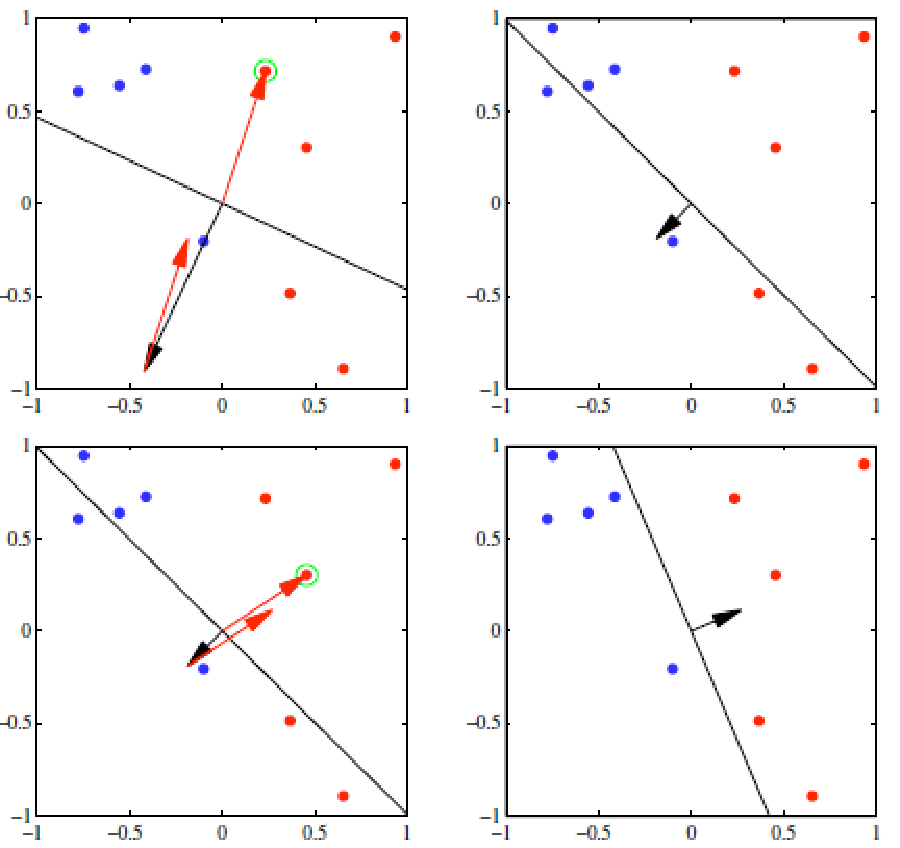
\includegraphics[width=12cm]{figure/fig32.pdf}
\end{center}
\caption{Perceptron learning iterations.}
\label{f:perceptron}
\end{figure}

%\medskip
%\centerline{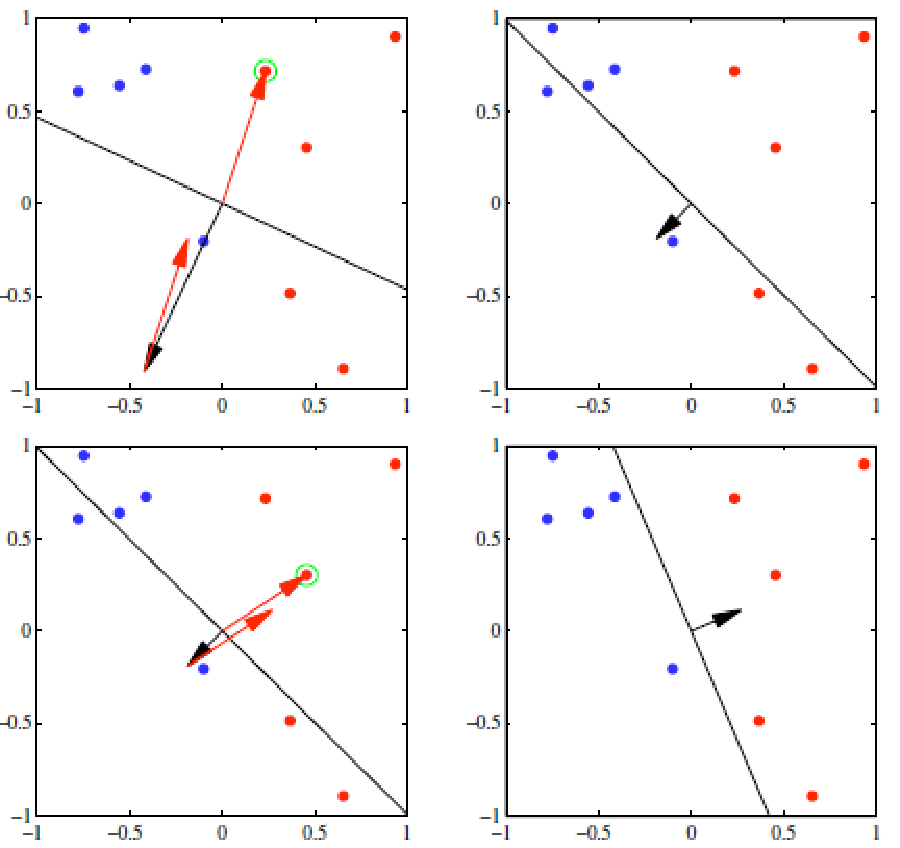
\includegraphics[width=0.5\textwidth]{figure/fig32.pdf}}

In Figure \ref{f:perceptron}, the black line represents the decision boundary associated with the current parameter vector $\w$ (ignoring the bias for simplicity), while the red vector corresponds to a misclassified input $\x_i$. When such a point is encountered, the algorithm modifies $\w$ by adding a scaled version of $\x_i$, effectively rotating the decision boundary in a direction that tends to correct the error.

At each step, if $\x_{i}$ is correctly classified, the weight vector remains unchanged. If instead it is misclassified, the contribution of $\x_i$ to the cost decreases after the update:
\begin{myalign}
-\x_{i}^T\w^{(k+1)}t_i&=-\x_{i}^T\w^{(k)}t_i-\eta(\x_{i}t_i)^{T}\x_{i}t_i\\
&=-\x_{i}^T\w^{(k)}t_i-\eta ||\x_i||^2\\
&<-\x_{i}^T\w^{(k)}t_i.
\end{myalign}
A similar argument holds when a bias term is included, leading to
\begin{myequation}
-\ox_{i}^T\ow^{(k+1)}t_i<-\ox_{i}^T\ow^{(k)}t_i.
\end{myequation}

This shows that the cost associated with the specific misclassified point $\x_i$ always decreases after an update. However, this does not guarantee that the total cost decreases at every iteration, since correcting one point might cause another point, previously classified correctly, to become misclassified.

Despite this, an important theoretical result states that if the two classes are linearly separable, the perceptron learning algorithm is guaranteed to converge to a separating hyperplane in a finite number of steps.

\medskip
To sketch the idea behind the convergence proof, let $\ow^*$ be a solution that correctly separates $C_{1}$ and $C_{2}$. If $\x_{k+1}$ is the point considered at iteration $(k+1)$ and it is misclassified, then the update satisfies
\begin{myequation}
\ow^{(k+1)}-\alpha{\hat \ow}=(\ow^{(k)}-\alpha{\hat \ow})+\eta\ox_{k+1}t_{k+1},
\end{myequation}
where $\alpha>0$ is a suitably chosen constant and $\hat\ow$ is a normalized version of $\ow^*$. This relation is used in the formal proof to show that the angle between $\ow^{(k)}$ and $\ow^*$ decreases over time, ultimately leading to convergence.

\medskip
\subsection*{Convergence of the Perceptron Algorithm}

We now present a detailed and intuitive proof of the convergence of the perceptron learning algorithm under the fundamental assumption that the two classes are linearly separable. Beyond merely showing that convergence occurs in a finite number of steps, we will derive an explicit bound on the number of updates required, revealing how the geometry of the data fundamentally determines the learning complexity. The elegance of this proof lies in its geometric intuition: we will track how the weight vector evolves through the parameter space, measuring its growing alignment with an optimal separating hyperplane while carefully controlling its magnitude.

\medskip
%\subsubsection*{Assumptions and Notation}

Before diving into the technical argument, let us establish the precise setting in which our result holds. We assume that the training set is linearly separable, which means geometrically that there exists at least one hyperplane capable of perfectly distinguishing between the two classes. Algebraically, this translates to the existence of a vector $\ow^*$ such that
\begin{myequation}
\ow^{*T}\ox_i t_i > 0 \quad \text{for all } i.
\end{myequation}

%Here, $\ox_i$ represents the $i$-th training example and $t_i \in \{-1, +1\}$ denotes its corresponding class label. 
The condition states that every training point lies on the correct side of the hyperplane defined by $\ow^*$, with the sign of the inner product matching the target label.

Without loss of generality, we normalize $\ow^*$ so that $\|\ow^*\|=1$. This normalization is purely conventional and simplifies the subsequent calculations by eliminating the scale ambiguity inherent in the definition of the separating hyperplane. We then define the \alert{margin} $\gamma>0$ as
\begin{myequation}
\gamma = \min{i} \ow^{*T}\ox_i t_i.
\end{myequation}
The margin carries deep geometric significance: it measures the minimum distance from any training point to the separating hyperplane, scaled by the norm of $\ow^*$. A larger $\gamma$ indicates that the classes are well-separated with substantial clearance from the decision boundary, suggesting an easier classification problem. Conversely, as $\gamma$ approaches zero, the classes become nearly touching, making the separation increasingly delicate. This quantity will emerge as the crucial parameter governing the speed of convergence.

We also define
\begin{myequation}
R = \max{i} \|\ox_i\|,
\end{myequation}
which represents the maximum norm of any training example. This parameter essentially captures the ``radius'' of the data cloud, bounding how far any point extends from the origin in the feature space. Together, $R$ and $\gamma$ characterize the intrinsic geometry of the learning problem, and their ratio will determine the worst-case number of updates the perceptron might require.

\medskip
%\paragraph*{The Key Insight Behind the Proof}

With our notation established, we can now articulate the central intuition driving the convergence proof. As deecsribed above, the learning algorithm begins with some initial weight vector $\ow^{(0)}$ (often the zero vector) and iteratively updates it whenever a misclassification is encountered. We wish to understand how this evolving weight vector $\ow^{(k)}$ relates to our ideal separator $\ow^*$ after $k$ updates.

The fundamental insight is twofold. First, every time the perceptron makes an update due to a misclassified example, the weight vector shifts in a direction that increases its agreement with $\ow^*$. This means the angle between $\ow^{(k)}$ and $\ow^*$ tends to decrease, or equivalently, their inner product grows. Second, while the alignment with $\ow^*$ increases steadily, the norm of $\ow^{(k)}$ cannot grow arbitrarily fast; its growth is constrained by the magnitude of the updates. 

To formalize this intuition, we analyze two complementary quantities throughout the learning trajectory. The first is the projection of $\ow^{(k)}$ onto $\ow^*$, given by the inner product $\ow^{(k)T}\ow^*$, which measures the alignment between the current hypothesis and the optimal separator. The second is the squared norm $\|\ow^{(k)}\|^2$, which tracks how large the weight vector becomes. %The interplay between these quantities - linear growth in alignment versus sublinear growth in magnitude - creates a tension that can only be sustained for a finite number of steps, thereby guaranteeing convergence.

\medskip
\subsubsection*{Growth of Alignment with the Optimal Separator}

Let us formalize more precisely how the alignment evolves. Suppose that item $\ox_{k+1}, t_{k+1}$ considered the algorithm at iteration $k$ is misclassified, that is $\ow^{(k)T}\ox_{k+1} t_{k+1} < 0$. In response, weights are updated as
\begin{myequation}
\ow^{(k+1)} = \ow^{(k)} + \eta \ox_{k+1} t_{k+1},
\end{myequation}
To assess how this update affects the alignment with $\ow^*$, we examine the inner product between the new weight vector and the optimal separator:
\begin{myalign}
\ow^{(k+1)T}\ow^* 
&= (\ow^{(k)} + \eta \ox_{k+1} t_{k+1})^T \ow^* \\
&= \ow^{(k)T}\ow^* + \eta\, \ox_{k+1}^T \ow^* t_{k+1}.
\end{myalign}
\begin{myalign}
\ow^{*T}\ow^{(k+1)}
&= \ow^{*T} (\ow^{(k)} + \eta \ox_{k+1} t_{k+1}) \\
&= \ow^{*T}\ow^(k)  + \eta\, \ow^{*T}\ox_{k+1} t_{k+1}.
\end{myalign}
This decomposition reveals that the new alignment equals the old alignment plus a correction term. The crucial observation is that, despite $\ox_{k+1}$ being misclassified by the current hypothesis $\ow^{(k)}$, it is correctly classified by the optimal hypothesis $\ow^*$. By definition of the margin $\gamma$, we know that
\begin{myequation}
\ox_{k+1}^T \ow^* t_{k+1} \ge \gamma,
\end{myequation}
since $\gamma$ represents the minimum value of this quantity across all training points. Substituting this bound yields
\begin{myequation}
\ow^{(k+1)T}\ow^* \ge \ow^{(k)T}\ow^* + \eta \gamma.
\end{myequation}
This inequality is powerful: it demonstrates that every single update increases the alignment with $\ow^*$ by at least $\eta\gamma$, regardless of which specific point triggered the update. 

Applying this argument recursively, we can trace the accumulation of these incremental gains. If we assume for simplicity that $\ow^{(0)} = \mathbf{0}$ (the typical initialization), then after $T$ updates we obtain
\begin{myequation}
\ow^{(T)T}\ow^* \ge T\,\eta\,\gamma.
\end{myequation}
Thus, the alignment between the learned weight vector and the optimal separator grows at least linearly with the number of updates. This linear lower bound reflects the consistent progress made toward the correct classification geometry with each mistake corrected.

\medskip
\subsubsection*{Controlled Growth of the Weight Vector Norm}

While the alignment with $\ow^*$ grows steadily, we must also understand how the magnitude of $\ow^{(k)}$ evolves. If the weight vector grew too rapidly, the increasing alignment might merely reflect inflation of the vector's scale rather than genuine directional improvement. We now show that such uncontrolled growth does not occur.

Beginning again from the update rule and computing the squared norm, we expand:
\begin{myalign}
\|\ow^{(k+1)}\|^2 
&= \|\ow^{(k)} + \eta \ox_{k+1} t_{k+1}\|^2 \\
&= \|\ow^{(k)}\|^2 + 2\eta\, \ow^{(k)T}\ox_{k+1} t_{k+1} + \eta^2 \|\ox_{k+1}\|^2.
\end{myalign}
This expansion contains three terms: the previous squared norm, a cross-term involving the current prediction, and the squared magnitude of the update direction. Here we encounter a critical observation: since $\ox_{k+1}$ is misclassified by $\ow^{(k)}$, we have $\ow^{(k)T}\ox_{k+1} t_{k+1} < 0$. This means the middle term is strictly negative (or zero in degenerate cases), representing the fact that the current hypothesis disagrees with the label. Consequently, dropping this negative term provides a valid upper bound:
\begin{myequation}
\|\ow^{(k+1)}\|^2 \le \|\ow^{(k)}\|^2 + \eta^2 \|\ox_{k+1}\|^2.
\end{myequation}
Recalling our definition of $R$ as the maximum norm of any training example, we can further bound $\|\ox_{k+1}\|^2 \le R^2$, yielding
\begin{myequation}
\|\ow^{(k+1)}\|^2 \le \|\ow^{(k)}\|^2 + \eta^2 R^2.
\end{myequation}
This recursive relation shows that the squared norm grows by at most $\eta^2 R^2$ with each update. Accumulating these increments over $k$ updates starting from $\ow^{(0)} = \mathbf{0}$ gives
\begin{myequation}
\|\ow^{(k)}\|^2 \le k\,\eta^2 R^2.
\end{myequation}
Thus, the norm grows at most as the square root of the number of updates, specifically $\|\ow^{(k)}\| \le \sqrt{k}\,\eta R$. This sublinear growth stands in marked contrast to the linear growth of the alignment, and it is precisely this disparity that will force convergence in finite time.

\medskip
\subsubsection*{Combining the Bounds to Establish Convergence}

We now possess two complementary descriptions of the weight vector after $k$ updates: a lower bound on its alignment with $\ow^*$ and an upper bound on its magnitude. The final step involves bringing these together through a fundamental geometric inequality.

The Cauchy--Schwarz inequality provides the necessary link, stating that for any two vectors, the inner product is bounded by the product of their norms:
\begin{myequation}
\ow^{(T)T}\ow^* \le \|\ow^{(T)}\|\,\|\ow^*\|.
\end{myequation}
Given our normalization $\|\ow^*\|=1$, this simplifies to $\ow^{(k)T}\ow^* \le \|\ow^{(k)}\|$. This inequality expresses the geometric fact that the projection of $\ow^{(k)}$ onto $\ow^*$ cannot exceed the length of $\ow^{(k)}$ itself.

Substituting our previously derived bounds into this inequality yields a remarkable constraint:
\begin{myequation}
k\,\eta\,\gamma \le \|\ow^{(k)}\| \le \sqrt{k}\,\eta R.
\end{myequation}
The left inequality comes from our alignment analysis, while the right inequality follows from our norm bound. Squaring both sides of the compound inequality eliminates the square root and gives
\begin{myequation}
k^2 \eta^2 \gamma^2 \le k \eta^2 R^2.
\end{myequation}
Assuming $k > 0$ (the case $k=0$ is trivial as no updates means immediate convergence), we can divide both sides by $k\eta^2$ to obtain the final result:
\begin{myequation}
k \le \left(\frac{R}{\gamma}\right)^2.
\end{myequation}
This elegant bound reveals that the number of updates $k$ required for convergence is fundamentally limited by the squared ratio of the data radius to the margin. Once the number of updates exceeds $(R/\gamma)^2$, the inequalities become contradictory, meaning no further misclassifications can occur and the algorithm must have converged to a separating hyperplane.

\medskip
\subsubsection*{Interpretation and Geometric Insight}

The Perceptron Convergence Theorem offers several profound insights into the nature of learning from data. Most importantly, it guarantees that the number of updates required for convergence is finite, ensuring that the algorithm will eventually find a separating hyperplane if one exists. This finiteness stands in contrast to many optimization procedures that might only approach a solution asymptotically.

The bound's dependence on $R$ and $\gamma$ reveals how the intrinsic geometry of the classification problem dictates learning complexity. When the margin $\gamma$ is large relative to the data scale $R$, indicating well-separated classes with generous clearance from the decision boundary, convergence occurs rapidly. The perceptron quickly discovers a satisfactory hypothesis because the updates consistently push the weight vector in directions that rapidly correct the classification geometry. Conversely, when the margin is small, suggesting classes that nearly touch or overlap slightly in the training set (though remaining separable), the learning process may require many more steps. The algorithm must navigate increasingly delicate adjustments to find a hyperplane that threads the narrow gap between classes.

Perhaps most remarkably, the bound is completely independent of the dimensionality of the feature space and of the total number of training points. Whether the data lives in ten dimensions or ten thousand, and whether the training set contains hundreds or millions of examples, the worst-case number of updates depends only on the margin and the maximum norm. %This dimension-free property foreshadows modern developments in statistical learning theory, where margin-based analysis has become central to understanding generalization in high-dimensional spaces.

It is worth noting that while the bound provides a worst-case guarantee, the actual number of updates observed in practice may be considerably smaller. The bound assumes that every update contributes minimally to alignment (exactly $\eta\gamma$) while maximally increasing the norm, a pessimistic scenario that need not reflect typical learning trajectories. Nevertheless, the existence of any finite bound, and particularly one with such clear geometric interpretation, establishes the perceptron as a theoretically well-founded learning algorithm.

\medskip
\subsubsection*{Final Remarks}

The perceptron learning algorithm thus provides a conceptually simple yet theoretically sound procedure for finding linear separators in the separable case. Its convergence guarantee illustrates how geometric intuition can yield powerful algorithmic insights. The explicit bound on convergence steps, depending solely on the margin and data radius, anticipates modern margin-based learning theory by several decades.

However, this elegant picture comes with important caveats. The theorem assumes linear separability, a condition that rarely holds exactly in real-world data contaminated by noise or arising from inherently non-linear relationships. When the data are not linearly separable, the perceptron algorithm loses its convergence guarantee and may oscillate indefinitely, cycling through a sequence of weight vectors without settling on a stable solution. This limitation motivated the development of more sophisticated approaches, such as support vector machines (which explicitly maximize the margin), and multilayer neural networks (which learn non-linear decision boundaries). 




%\end{document}